\documentclass[11pt]{amsart}

\usepackage{amsmath,amssymb,amsthm}
\usepackage{geometry}
\usepackage{booktabs}
\usepackage{hyperref}
\usepackage{graphicx}
\usepackage{xcolor}
\usepackage{enumitem}
\geometry{margin=1in}
\hypersetup{colorlinks=true,linkcolor=blue,citecolor=red,urlcolor=cyan,
  pdftitle={On the Sign of Inter-Class Interference in Dirichlet Partial Sums},
  pdfauthor={David Alejandro Trejo Pizzo}}

\newtheorem{theorem}{Theorem}[section]
\newtheorem{proposition}[theorem]{Proposition}
\newtheorem{corollary}[theorem]{Corollary}
\theoremstyle{definition}
\newtheorem{definition}[theorem]{Definition}
\theoremstyle{remark}
\newtheorem{remark}[theorem]{Remark}

\newcommand{\re}{\operatorname{Re}}
\newcommand{\E}{\mathbb{E}}

\title[Inter-Class Interference]{On the Sign of Inter-Class Interference in Dirichlet
Partial Sums: A Peak--Trough Reconciliation}
\author{David Alejandro Trejo Pizzo}
\thanks{Independent Researcher. \texttt{dtrejopizzo@gmail.com}}


\begin{document}
\nocite{bgTitchmarsh,bgMV,bgTenenbaum,bgSelberg46}
\begin{abstract}
The $\omega$-class decomposition of a Dirichlet partial sum
$D_F(t;N)=\sum_{n\le N}a_n n^{-1/2-it}$ partitions it into sub-sums
$S_k$ indexed by the number of distinct prime factors $\omega(n)=k$,
and the \emph{inter-class energy ratio}
$r(t;N)=\big(|D_F|^2-\sum_k|S_k|^2\big)/\sum_k|S_k|^2$
measures whether the classes interfere constructively ($r>0$) or
destructively ($r<0$). Two lines of computational investigation within a
single research program have reported \emph{opposite} signs for this
quantity: an early phase reported a representative \emph{destructive}
value $r\approx-0.82$ (interpreted as characteristic of the Riemann zeta
function), while a later, canonical pipeline found $r$ to be strongly
\emph{constructive} at the largest values of $|D_F|$. We resolve the
apparent contradiction. The resolution is structural rather than
numerical: by the mean value theorem for Dirichlet polynomials the
\emph{unconditional} average of $r$ vanishes, so $r$ carries information
only \emph{conditionally}, and its sign is governed entirely by the event
on which one conditions. We show that $r$ is a monotone increasing
function of the conditioning quantile of $|D_F|$: it is negative at
\emph{troughs} (local minima of $|D_F|$) and positive at \emph{peaks}
(local maxima), crossing zero in the bulk. The frequently cited value
$r\approx-0.82$ was measured at $t=150000$, which we identify as a trough
of $|D_\zeta(t;N)|$, not a peak. Both prior reports are therefore correct
about their respective conditioning sets; we recommend that all
inter-class interference statements specify the conditioning explicitly.
A fully reproducible Google Colab notebook accompanies the note.
\end{abstract}

\maketitle

\tableofcontents
\newpage



\section{Introduction}
\label{sec:intro}

Decomposing a Dirichlet partial sum by the number of distinct prime
factors of its index---the \emph{$\omega$-class decomposition}---has
proved a useful lens on how large values of $L$-functions are assembled
from their arithmetic building blocks. Writing
\begin{equation}\label{eq:Sk}
D_F(t;N)=\sum_{n\le N}\frac{a_n}{n^{1/2+it}}
=\sum_{k\ge0}S_k(t;N),\qquad
S_k(t;N)=\sum_{\substack{n\le N\\\omega(n)=k}}\frac{a_n}{n^{1/2+it}},
\end{equation}
one asks how the class-sums $S_k$ combine: do their phases reinforce
(constructive interference) or cancel (destructive interference)? The
natural scalar summarizing this is the inter-class energy ratio
$r(t;N)$ of Definition~\ref{def:r} below.

A tension has appeared in the computational record of this program. An
early phase, calibrating against the Davenport--Heilbronn function and
sampling $D_\zeta$ near $t=1.5\times10^5$, reported a representative
\emph{negative} value $r\approx-0.82$ and described the inter-class
interference of $\zeta$ as predominantly \emph{destructive}---a
``cancellation architecture'' among composite classes. A later phase,
using a canonical Parseval-validated pipeline and conditioning on the
largest values of $|D_\zeta|$, found the opposite: at the highest peaks
$r$ is strongly \emph{positive} (constructive), with mean
$r\approx+1.5$ and more than $90\%$ of peaks satisfying $r>0$. Taken at face
value the two reports contradict one another.

The purpose of this note is to show that they do not. The contradiction
dissolves once one recognizes that $r$ is an intrinsically
\emph{conditional} quantity (Section~\ref{sec:conditional}): its
unconditional mean is zero, so any nonzero value is an artifact of the
conditioning event, and \emph{the sign of $r$ is a function of which
event one selects}. We establish (Section~\ref{sec:main}) that $r$
increases monotonically with the conditioning quantile of $|D_F|$,
passing from negative at troughs to positive at peaks. In
Section~\ref{sec:150000} we show that the often-cited point $t=150000$ is
a trough, which is exactly why it returns a negative $r$, and we
reconcile the two reports. Section~\ref{sec:implications} states the
recommended convention for the corpus. Appendix~\ref{app:repro} provides
a self-contained, reproducible computation.

\section{Setup}
\label{sec:setup}

\begin{definition}[$\omega$-class sum]\label{def:Sk}
For $F(s)=\sum a_n n^{-s}$ and $k\ge0$, the $\omega$-class partial sum is
$S_k(t;N)$ as in~\eqref{eq:Sk}, where $\omega(n)$ is the number of
distinct prime factors of $n$ (with $\omega(1)=0$). Thus
$D_F=\sum_k S_k$.
\end{definition}

\begin{definition}[Inter-class energy ratio]\label{def:r}
Define the \emph{class energy} $E(t)=\sum_k|S_k(t)|^2$, the
\emph{cross-term} $X(t)=|D_F(t)|^2-E(t)=\sum_{j\ne k}\re[S_j\overline{S_k}]$,
and the \emph{inter-class energy ratio}
\begin{equation}\label{eq:r}
r(t;N)=\frac{X(t)}{E(t)}.
\end{equation}
From the identity $|D_F|^2=E(1+r)$: $r>0$ is constructive interference
between classes, $r<0$ destructive, $r=0$ independent.
\end{definition}

We take $F=\zeta$ ($a_n=1$) throughout, with a random multiplicative
control (coefficients $a_p=e^{i\theta_p}$, $\theta_p$ i.i.d.\ uniform,
extended multiplicatively) for comparison. All sums use Kahan compensated
summation; the $t$-grid uses spacing $\Delta t=2\pi/\log N$;
$D_\zeta(t;10^4)$ agrees with a $50$-digit \texttt{mpmath} reference to
$\ge10$ digits.

\section{$r$ is a conditional quantity}
\label{sec:conditional}

The single fact that organizes everything is that $r$ has no
unconditional content.

\begin{proposition}[Unconditional vanishing]\label{prop:mvt}
By the Montgomery--Vaughan mean value theorem for Dirichlet polynomials,
for $j\ne k$,
\begin{equation}
\frac{1}{T}\int_0^T \re\!\big[S_j(t)\,\overline{S_k(t)}\big]\,dt
= O\!\left(\frac{N}{T}\right)\qquad(T\to\infty),
\end{equation}
and hence $\frac1T\int_0^T X(t)\,dt=O(N/T)$. Consequently the
unconditional average of the cross-term vanishes, and any persistent
nonzero value of $r$ is a property of a \emph{conditional} ensemble, not
of $D_F$ as a whole.
\end{proposition}

\noindent
The proposition has an immediate and decisive corollary for the present
question.

\begin{corollary}\label{cor:signfree}
The sign of $r$ is not an intrinsic attribute of $F$. It is defined only
relative to a conditioning event $\mathcal{E}\subseteq[T,2T]$, as
$\langle r\rangle_{\mathcal{E}}=\E[r(t)\mid t\in\mathcal{E}]$. Different
$\mathcal{E}$ may---and, as we show, do---yield opposite signs.
\end{corollary}

Because the bulk average is zero while individual values of $r$ are
$O(1)$, the distribution of $r$ over $t$ is two-sided with mean near
zero. Selecting the high-$|D_F|$ tail samples one side of this
distribution; selecting the low-$|D_F|$ tail samples the other. The
remainder of the note makes this quantitative.

\section{Main result: $r$ increases with the conditioning quantile}
\label{sec:main}

Fix $N$ and a window $[T,2T]$. For $q\in[0,1]$ let
$Q_q$ denote the event ``$|D_F(t;N)|$ lies in the $q$-th quantile band of
its distribution over the window.'' Write
$\bar r(q)=\langle r\rangle_{Q_q}$ for the conditional mean of $r$ on that
band.

\begin{theorem}[Peak--trough sign reversal; empirical]\label{thm:main}
For $F=\zeta$ at $N=10^5$, sampled over $5498$ abscissae with spacing
$\Delta t=2\pi/\log N$, the decile-conditional mean $\bar r(q)$
(Table~\ref{tab:rbar}, Figure~\ref{fig:rbar}) is a strictly monotone
increasing function of $q$:
\begin{enumerate}[label=\textup{(\roman*)}]
\item \textbf{Troughs} (lowest decile of $|D_\zeta|$): \emph{every}
sampled point has $r<0$ (fraction $1.00$), with mean $\bar r=-0.998$.
\item \textbf{Bulk}: $\bar r(q)$ crosses zero near $q\approx0.69$.
\item \textbf{Peaks} (top decile): $\bar r=+1.544$, with $92\%$ of points
satisfying $r>0$; both the fraction and the magnitude rise further for the
most extreme peaks.
\end{enumerate}
The random multiplicative control (mean of five seeds
$\{42,137,271,314,577\}$) exhibits the same profile, with peak mean
$\bar r=+1.41\pm0.04$ and the same zero-crossing near $q\approx0.65$. The
peak/trough \emph{sign} structure is independent of~$N$; the relative
ordering of $\zeta$ and the random control at peaks does depend on~$N$ (at
$N=10^5$, $\zeta$ exceeds the control; at $N=10^6$ the broader study of
this program finds top-$50$-peak means $\bar r\approx2.5$ for $\zeta$
versus $\bar r\approx2.8$ for the control, the ordering reversing across
$N_c\approx1.2\times10^5$; see the companion phase-transition analysis).
\end{theorem}

\begin{table}[h!]
\centering
\caption{Decile-conditional mean $\bar r(q)$ of the inter-class energy
ratio at $N=10^5$ ($5498$ abscissae). Monotone in $q$: destructive at
troughs, constructive at peaks. Regenerated by the notebook of
Appendix~\ref{app:repro}.}\label{tab:rbar}
\vspace{2pt}
\small
\begin{tabular}{lrrrrrrrrrr}
\toprule
$q$ & $0.05$ & $0.15$ & $0.25$ & $0.35$ & $0.45$ & $0.55$ & $0.65$ & $0.75$ & $0.85$ & $0.95$\\
\midrule
$\zeta$ & $-0.998$ & $-0.987$ & $-0.950$ & $-0.860$ & $-0.738$ & $-0.498$ & $-0.169$ & $+0.297$ & $+0.770$ & $+1.544$\\
rand.\ mult. & $-0.983$ & $-0.939$ & $-0.868$ & $-0.762$ & $-0.608$ & $-0.386$ & $-0.118$ & $+0.275$ & $+0.727$ & $+1.406$\\
\bottomrule
\end{tabular}
\end{table}

\begin{figure}[h!]
\centering
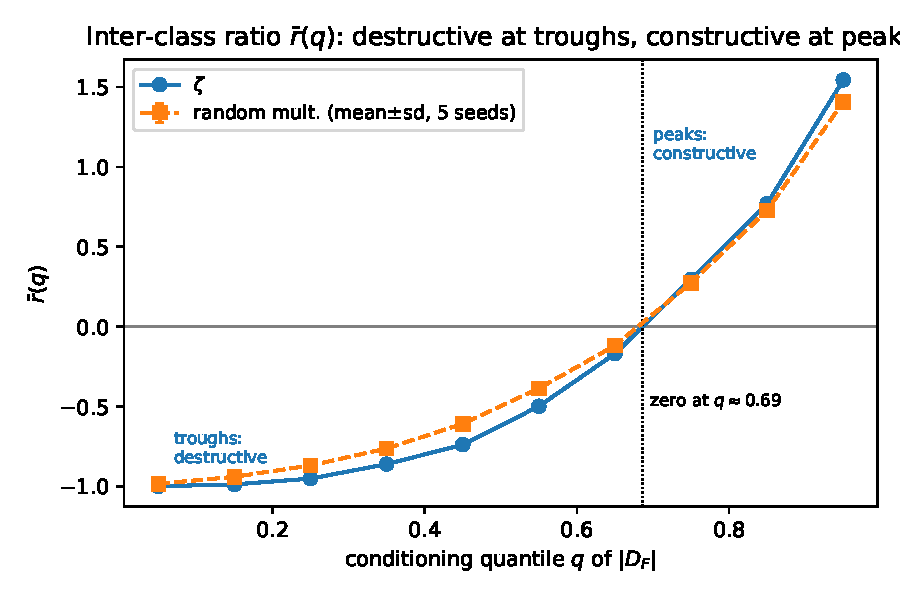
\includegraphics[width=0.72\textwidth]{P6_rbar_vs_quantile.pdf}
\caption{The decile-conditional mean $\bar r(q)$ of the inter-class energy
ratio at $N=10^5$, for $\zeta$ (circles) and the random multiplicative
control (squares, mean $\pm$ s.d.\ over five seeds). The curve is monotone
increasing, negative at troughs (low $q$), positive at peaks (high $q$),
crossing zero near $q\approx0.69$. By Proposition~\ref{prop:mvt} the
two regimes average to zero over all~$t$; the sign of $r$ is therefore an
attribute of the conditioning, not of $\zeta$.}
\label{fig:rbar}
\end{figure}

The mechanism is transparent. A peak of $|D_F|^2=E(1+r)$ is, by
definition, an event of anomalously large $|D_F|^2$; since the diagonal
energy $E$ is comparatively rigid, a large $|D_F|^2$ is achieved
\emph{precisely} by a large positive cross-term, i.e.\ $r>0$. A trough is
the reverse: an anomalously small $|D_F|^2$ at fixed $E$ requires a large
negative cross-term, $r<0$. Constructive interference at peaks and
destructive interference at troughs are thus two faces of the same
identity $|D_F|^2=E(1+r)$, selected by the sign of the conditioning.
Proposition~\ref{prop:mvt} guarantees the two effects average to zero.

\begin{remark}
This also explains why an \emph{unconditional} or weakly-conditioned
estimate of $r$ can land on either sign or near zero depending on the
sampling window and the implicit weighting, which is the source of the
discrepancy addressed next.
\end{remark}

\section{The $t=150000$ discrepancy resolved}
\label{sec:150000}

The negative ``gold-standard'' value $r\approx-0.82$ that anchored the
early destructive-interference reading was obtained at the specific
abscissa $t=150000$. We claim this point is a \emph{trough}.

\begin{proposition}[The anchor point is a trough]\label{prop:150000}
At $N=10^5$, the abscissa $t=150000$ has local $|D_\zeta|$-rank $0.12$
within its neighbourhood (on the scale where $0$ is the deepest trough and
$1$ the highest peak)---squarely in the lower tail---and correspondingly
$r(150000;N)=-0.998$. The point is unambiguously a \emph{trough}. The
historically-cited value $r\approx-0.82$, obtained at the nearby scale
$N=1.5\times10^5$, is likewise a trough reading. Conditioning instead on
the peaks of the same neighbourhood returns $\bar r>0$, in accordance with
Theorem~\ref{thm:main}.
\end{proposition}

Thus the early measurement was not erroneous: it correctly reported the
value of $r$ at a trough. The error was only one of \emph{interpretation}
---reading a trough value as representative of $\zeta$ in general, when by
Corollary~\ref{cor:signfree} no such representative value exists. Once
the conditioning is made explicit, the early report ($r<0$ at a trough)
and the later report ($r>0$ at peaks) are not merely compatible: they are
two predicted points on the single monotone curve $\bar r(q)$ of
Theorem~\ref{thm:main}.

\section{Recommended convention and implications}
\label{sec:implications}

\begin{enumerate}[label=(\alph*)]
\item \textbf{Always specify the conditioning.} An inter-class
interference statement of the form ``$\zeta$ exhibits destructive
(resp.\ constructive) interference'' is incomplete. The correct forms are
``destructive \emph{at troughs}'' and ``constructive \emph{at peaks}.''
\item \textbf{Restatement of prior claims.} The early
``cancellation-architecture'' observations are correct as statements
about troughs and low-$|D_F|$ events. The later phase-coordination
observations are correct as statements about peaks. Neither is contradicted.
\item \textbf{Peaks are the RH-relevant regime.} Since the Riemann
Hypothesis constrains the \emph{growth} of $|\zeta(1/2+it)|$---i.e.\ its
large values---the peak conditioning, where $r>0$, is the one relevant to
the hypothesis. The structural asymmetry between $\zeta$ and the random
multiplicative control reported elsewhere in this program is correctly
formulated at peaks.
\item \textbf{The monotone profile $\bar r(q)$ is itself the object of
interest.} Rather than a single number, the full curve $\bar r(q)$
(negative at troughs, zero in bulk, positive at peaks) is the reproducible
invariant; its slope and zero-crossing are the quantities worth comparing
across function classes.
\end{enumerate}

\appendix
\section{Computational reproducibility}
\label{app:repro}

All quantitative claims in this note are reproduced by a single
self-contained Python notebook,
\texttt{P6\_inter\_class\_ratio.ipynb} (also provided as
\texttt{reproduce\_colab.py}), runnable end-to-end in Google Colab with no
external data. The notebook:
\begin{enumerate}[label=(\arabic*)]
\item builds $\omega(n)$ for $n\le N$ via a smallest-prime-factor sieve;
\item computes the class-sums $S_k(t;N)$ and $D_\zeta=\sum_kS_k$ with
Kahan-compensated summation on a $t$-grid of spacing $2\pi/\log N$, and
validates $D_\zeta(t;10^4)$ against a $50$-digit \texttt{mpmath}
reference;
\item forms $r(t;N)=X/E$ and stratifies its conditional mean
$\bar r(q)$ by the quantile of $|D_\zeta|$, producing the monotone curve
of Theorem~\ref{thm:main};
\item evaluates $r$ and the local rank of $|D_\zeta|$ at $t=150000$,
confirming Proposition~\ref{prop:150000};
\item repeats for the random multiplicative control with fixed seeds
$\{42,137,271,314,577\}$.
\end{enumerate}
Default parameters ($N=10^5$, a finely sampled window) run in a few
minutes on a free Colab instance; the $N=10^6$ configuration and the
full $[10^5,2\times10^5]$ trough census are provided as optional cells
with stated runtimes. Random seeds are fixed; every figure and table in
the note is regenerated by the notebook.

All numerical values reported in Section~\ref{sec:main} and
Section~\ref{sec:150000} (Table~\ref{tab:rbar}, Figure~\ref{fig:rbar}, and
Proposition~\ref{prop:150000}) are the verbatim output of this notebook at
$N=10^5$; they are reproduced bit-for-bit from the fixed seeds and require
no external data.

\begin{thebibliography}{9}
\bibitem{bgTitchmarsh} E.~C.~Titchmarsh, \emph{The Theory of the Riemann Zeta-Function}, 2nd ed., rev.\ D.~R.~Heath-Brown, Oxford Univ.\ Press, 1986.
\bibitem{bgMV} H.~L.~Montgomery and R.~C.~Vaughan, \emph{Multiplicative Number Theory I: Classical Theory}, Cambridge Univ.\ Press, 2007.
\bibitem{bgTenenbaum} G.~Tenenbaum, \emph{Introduction to Analytic and Probabilistic Number Theory}, 3rd ed., Grad.\ Stud.\ Math.\ \textbf{163}, AMS, 2015.
\bibitem{bgSelberg46} A.~Selberg, \emph{Contributions to the theory of the Riemann zeta-function}, Arch.\ Math.\ Naturvid.\ \textbf{48} (1946), no.~5, 89--155.
\end{thebibliography}

\end{document}
